\documentclass[10pt,oneside]{article}
\usepackage[T1]{fontenc}
\usepackage[utf8]{inputenc}
% \usepackage{lmodern}
%\usepackage[adobe-utopia,uppercase=upright,greeklowercase=upright]{mathdesign}
\usepackage[adobe-utopia]{mathdesign}
%\usepackage{minionpro}
% \usepackage{pifont}
% \usepackage{amssymb}
\usepackage{amsmath}
\usepackage[francais]{babel}
% \usepackage[francais]{varioref}
\usepackage[dvips]{graphicx}

\usepackage{framed}
\usepackage[normalem]{ulem}
\usepackage{fancyhdr}
\usepackage{titlesec}
\usepackage{vmargin}
\usepackage{longtable}

\usepackage{ifthen}


%\usepackage{epsfig}
\usepackage{subfig}

\usepackage{multirow}
\usepackage{multicol} % Portions de texte en colonnes
\usepackage{flafter}%floatants après la référence



\usepackage{color}
\usepackage{colortbl}


\definecolor{gris25}{gray}{0.75}
\definecolor{bleu}{RGB}{18,33,98}
\definecolor{bleuf}{RGB}{42,94,171}
\definecolor{bleuc}{RGB}{231,239,247}
\definecolor{rougef}{RGB}{185,18,27}
\definecolor{rougec}{RGB}{255,230,231}
\definecolor{vertf}{RGB}{103,126,82}
\definecolor{vertc}{RGB}{220,255,191}
\definecolor{violetf}{RGB}{112,48,160}
\definecolor{violetc}{RGB}{230,224,236}

\newenvironment{sci}[1][\hsize]%
{%
    \def\FrameCommand%
    {%
%\rotatebox{90}{\textit{\textsf{Scilab}}\includegraphics[height=.8cm]{png/logo_scilab}} 
\rotatebox{90}{\includegraphics[height=.6cm]{png/logo_scilab}} 
        {\color{violetf}\vrule width 3pt}%
        \hspace{0pt}%must no space.
        \fboxsep=\FrameSep\colorbox{violetc}%
    }%
    \MakeFramed{\hsize #1 \advance\hsize-\width\FrameRestore}%
}%
{\endMakeFramed}%

\newenvironment{pseudo}[1][\hsize]%
{%
    \def\FrameCommand%
    {%
\rotatebox{90}{\textit{\textsf{Pseudo Code}}} 
        {\color{violetf}\vrule width 3pt}%
        \hspace{0pt}%must no space.
        \fboxsep=\FrameSep\colorbox{violetc}%
    }%
    \MakeFramed{\hsize #1 \advance\hsize-\width\FrameRestore}%
}%
{\endMakeFramed}%

\newenvironment{py}[1][\hsize]%
{%
    \def\FrameCommand%
    {%
%\rotatebox{90}{\textit{\textsf{Python}}} 
\rotatebox{90}{\includegraphics[height=.6cm]{png/logo_python}} 
        {\color{violetf}\vrule width 3pt}%
        \hspace{0pt}%must no space.
        \fboxsep=\FrameSep\colorbox{violetc}%
    }%
    \MakeFramed{\hsize #1 \advance\hsize-\width\FrameRestore}%
}%
{\endMakeFramed}%


\newenvironment{corrige}[1][\hsize]%
{%
    \def\FrameCommand
    {%
\rotatebox{90}{\textit{\textsf{Correction}}} 
        {\color{violetf}\vrule width 3pt}%
        \hspace{0pt}%must no space.
        \fboxsep=\FrameSep\colorbox{violetc}%
    }%
    \MakeFramed{\hsize#1\advance\hsize-\width\FrameRestore}%
}%
{\endMakeFramed}%



\newenvironment{rem}[1][\hsize]%
{%
    \def\FrameCommand
    {%
\rotatebox{90}{\textit{\textsf{Remarque}}} 
        {\color{bleuf}\vrule width 3pt}%
        \hspace{0pt}%must no space.
        \fboxsep=\FrameSep\colorbox{bleuc}%
    }%
    \MakeFramed{\hsize#1\advance\hsize-\width\FrameRestore}%
}%
{\endMakeFramed}%


\newenvironment{savoir}[1][\hsize]%
{%
    \def\FrameCommand
    {%
\rotatebox{90}{\textit{\textsf{Savoir}}} 
        {\color{bleuf}\vrule width 3pt}%
        \hspace{0pt}%must no space.
        \fboxsep=\FrameSep\colorbox{bleuc}%
    }%
    \MakeFramed{\hsize#1\advance\hsize-\width\FrameRestore}%
}%
{\endMakeFramed}%

\newenvironment{prob}[1][\hsize]%
{%
    \def\FrameCommand%
    {%
\rotatebox{90}{\textit{\textsf{ Problématique}}} 
        {\color{rougef}\vrule width 3pt}%
        \hspace{0pt}%must no space.
        \fboxsep=\FrameSep\colorbox{rougec}%
    }%
    \MakeFramed{\hsize#1\advance\hsize-\width\FrameRestore}%
}%
{\endMakeFramed}%

\newenvironment{obj}[1][\hsize]%
{%
    \def\FrameCommand%
    {%
\rotatebox{90}{\textit{\textsf{ $\;$}}} 
        {\color{rougef}\vrule width 3pt}%
        \hspace{0pt}%must no space.
        \fboxsep=\FrameSep\colorbox{rougec}%
    }%
    \MakeFramed{\hsize#1\advance\hsize-\width\FrameRestore}%
}%
{\endMakeFramed}%

\newenvironment{defi}[1][\hsize]%
{%
    \def\FrameCommand%
    {%
\rotatebox{90}{\textit{\textsf{Définition\\}}} 
        {\color{bleuf}\vrule width 3pt}%
        \hspace{0pt}%must no space.
        \fboxsep=\FrameSep\colorbox{bleuc}%
    }%
    \MakeFramed{\hsize#1\advance\hsize-\width\FrameRestore}%
}%
{\endMakeFramed}%


\newenvironment{demo}[1][\hsize]%
{%
    \def\FrameCommand%
    {%
\rotatebox{90}{\textit{\textsf{Démonstration\\}}} 
        {\color{bleuf}\vrule width 3pt}%
        \hspace{0pt}%must no space.
        \fboxsep=\FrameSep\colorbox{bleuc}%
    }%
    \MakeFramed{\hsize#1\advance\hsize-\width\FrameRestore}%
}%
{\endMakeFramed}%


\newenvironment{hypo}[1][\hsize]%
{%
    \def\FrameCommand%
    {%
\rotatebox{90}{\textit{\textsf{Hypothèse\\}}} 
        {\color{bleuf}\vrule width 3pt}%
        \hspace{0pt}%must no space.
        \fboxsep=\FrameSep\colorbox{bleuc}%
    }%
    \MakeFramed{\hsize#1\advance\hsize-\width\FrameRestore}%
}%
{\endMakeFramed}%


\newenvironment{prop}[1][\hsize]%
{%
    \def\FrameCommand%
    {%
\rotatebox{90}{\textit{\textsf{Propriété\\}}} 
        {\color{bleuf}\vrule width 3pt}%
        \hspace{0pt}%must no space.
        \fboxsep=\FrameSep\colorbox{bleuc}%
    }%
    \MakeFramed{\hsize#1\advance\hsize-\width\FrameRestore}%
}%
{\endMakeFramed}%

\newenvironment{props}[1][\hsize]%
{%
    \def\FrameCommand%
    {%
\rotatebox{90}{\textit{\textsf{Propriétés\\}}} 
        {\color{bleuf}\vrule width 3pt}%
        \hspace{0pt}%must no space.
        \fboxsep=\FrameSep\colorbox{bleuc}%
    }%
    \MakeFramed{\hsize#1\advance\hsize-\width\FrameRestore}%
}%
{\endMakeFramed}%

\newenvironment{exemple}[1][\hsize]%
{%
    \def\FrameCommand%
    {%
\rotatebox{90}{\textit{\textsf{Exemple\\}}} 
        {\color{vertf}\vrule width 3pt}%
        \hspace{0pt}%must no space.
        \fboxsep=\FrameSep\colorbox{vertc}%
    }%
    \MakeFramed{\hsize#1\advance\hsize-\width\FrameRestore}%
}%
{\endMakeFramed}%

\newenvironment{resultat}[1][\hsize]%
{%
    \def\FrameCommand%
    {%
\rotatebox{90}{\textit{\textsf{Résultat\\}}} 
        {\color{rougef}\vrule width 3pt}%
        \hspace{0pt}%must no space.
        \fboxsep=\FrameSep\colorbox{rougec}%
    }%
    \MakeFramed{\hsize#1\advance\hsize-\width\FrameRestore}%
}%
{\endMakeFramed}%

\newenvironment{methode}[1][\hsize]%
{%
    \def\FrameCommand%
    {%
\rotatebox{90}{\textit{\textsf{Méthode\\}}} 
        {\color{rougef}\vrule width 3pt}%
        \hspace{0pt}%must no space.
        \fboxsep=\FrameSep\colorbox{rougec}%
    }%
    \MakeFramed{\hsize#1\advance\hsize-\width\FrameRestore}%
}%
{\endMakeFramed}%

\newenvironment{theo}[1][\hsize]%
{%
    \def\FrameCommand%
    {%
\rotatebox{90}{\textit{\textsf{Théorème\\}}} 
        {\color{rougef}\vrule width 3pt}%
        \hspace{0pt}%must no space.
        \fboxsep=\FrameSep\colorbox{rougec}%
    }%
    \MakeFramed{\hsize#1\advance\hsize-\width\FrameRestore}%
}%
{\endMakeFramed}%

\newenvironment{warn}[1][\hsize]%
{%
    \def\FrameCommand%
    {%
\rotatebox{90}{\textit{\textsf{Attention\\}}} 
        {\color{rougef}\vrule width 3pt}%
        \hspace{0pt}%must no space.
        \fboxsep=\FrameSep\colorbox{rougec}%
    }%
    \MakeFramed{\hsize#1\advance\hsize-\width\FrameRestore}%
}%
{\endMakeFramed}%

% \usepackage{pstricks}
%\usepackage{minitoc}
% \setcounter{minitocdepth}{4}

\setcounter{tocdepth}{2}

% \mtcselectlanguage{french} 

%\usepackage{draftcopy}% "Brouillon"
% \usepackage{floatflt}
\usepackage{psfrag}
%\usepackage{listings} % Permet d'insérer du code de programmation
\renewcommand{\baselinestretch}{1.2}

% Changer la numérotation des figures :
% ------------------------------------
% \makeatletter
% \renewcommand{\thefigure}{\ifnum \c@section>\z@ \thesection.\fi
%  \@arabic\c@figure}
% \@addtoreset{figure}{section}
% \makeatother
 


%%%%%%%%%%%%
% Définition des vecteurs %
%%%%%%%%%%%%
 \newcommand{\vect}[1]{\overrightarrow{#1}}

%%%%%%%%%%%%
% Définition des torseusr %
%%%%%%%%%%%%

 \newcommand{\torseur}[1]{%
\left\{{#1}\right\}
}

\newcommand{\torseurcin}[3]{%
\left\{\mathcal{#1} \left(#2/#3 \right) \right\}
}

\newcommand{\torseurstat}[3]{%
\left\{\mathcal{#1} \left(#2\rightarrow #3 \right) \right\}
}

 \newcommand{\torseurc}[8]{%
%\left\{#1 \right\}=
\left\{
{#1}
\right\}
 = 
\left\{%
\begin{array}{cc}%
{#2} & {#5}\\%
{#3} & {#6}\\%
{#4} & {#7}\\%
\end{array}%
\right\}_{#8}%
}

 \newcommand{\torseurcol}[7]{
\left\{%
\begin{array}{cc}%
{#1} & {#4}\\%
{#2} & {#5}\\%
{#3} & {#6}\\%
\end{array}%
\right\}_{#7}%
}

 \newcommand{\torseurl}[3]{%
%\left\{\mathcal{#1}\right\}_{#2}=%
\left\{%
\begin{array}{l}%
{#1} \\%
{#2} %
\end{array}%
\right\}_{#3}%
}

 \newcommand{\vectv}[3]{%
\vect{V\left( {#1} \in {#2}/{#3}\right)}
}


\newcommand{\vectf}[2]{%
\vect{R\left( {#1} \rightarrow {#2}\right)}
}

\newcommand{\vectm}[3]{%
\vect{\mathcal{M}\left( {#1}, {#2} \rightarrow {#3}\right)}
}


 \newcommand{\vectg}[3]{%
\vect{\Gamma \left( {#1} \in {#2}/{#3}\right)}
}

 \newcommand{\vecto}[2]{%
\vect{\Omega\left( {#1}/{#2}\right)}
}
% }$$\left\{\mathcal{#1} \right\}_{#2} =%
% \left\{%
% \begin{array}{c}%
%  #3 \\%
%  #4 %
% \end{array}%
% \right\}_{#5}}

%  ------------------------------------------
% | Modification du formatage des sections : | 
%  ------------------------------------------

% Grands titres :
% ---------------

\newcommand{\titre}[1]{%
\begin{center}
      \bigskip
      \rule{\textwidth}{1pt}
      \par\vspace{0.1cm}
      
      \textbf{\large #1}
      \par\rule{\textwidth}{1pt}
    \end{center}
    \bigskip
  }

% Supprime le numéro du chapitre dans la numérotation des sections:
% -----------------------------------------------------------------
\makeatletter
\renewcommand{\thesection}{\@arabic\c@section}
\makeatother


% \titleformat{\chapter}[display]
% {\normalfont\Large\filcenter}
% {}
% {1pc}
% {\titlerule[1pt]
%   \vspace{1pc}%
%   \Huge}[\vspace{1ex}%
% \titlerule]


%%%% Chapitres Comme PY Pechard %%%%%%%%%
% numéro du chapitre
\DeclareFixedFont{\chapnumfont}{OT1}{phv}{b}{n}{80pt}
% pour le mot « Chapitre »
\DeclareFixedFont{\chapchapfont}{OT1}{phv}{m}{it}{40pt}
% pour le titre
\DeclareFixedFont{\chaptitfont}{T1}{phv}{b}{n}{25pt}

\definecolor{gris}{gray}{0.75}
\titleformat{\chapter}[display]%
	{\sffamily}%
	{\filleft\chapchapfont\color{gris}\chaptertitlename\
	\\
	\vspace{12pt}
	\chapnumfont\thechapter}%
	{16pt}%
	{\filleft\chaptitfont}%
	[\vspace{6pt}\titlerule\titlerule\titlerule]

%%%%  Fin Chapitres Comme PY Pechard %%%%%%%%%


% Section, subsection, subsubsection sans serifs :
% % ----------------------------------------------

% \makeatletter
% \renewcommand{\section}{\@startsection{section}{0}{0mm}%
% {\baselineskip}{.3\baselineskip}%
% {\normalfont\sffamily\Large\textbf}}%
% \makeatother

\makeatletter
\renewcommand{\@seccntformat}[1]{{\textcolor{bleu}{\csname
the#1\endcsname}\hspace{0.5em}}}
\makeatother

\makeatletter
\renewcommand{\section}{\@startsection{section}{1}{\z@}%
                       {-4ex \@plus -1ex \@minus -.4ex}%
                       {1ex \@plus.2ex }%
                       {\normalfont\Large\sffamily\bfseries}}%
\makeatother
 
\makeatletter
\renewcommand{\subsection}{\@startsection {subsection}{2}{\z@}
                          {-3ex \@plus -0.1ex \@minus -.4ex}%
                          {0.5ex \@plus.2ex }%
                          {\normalfont\large\sffamily\bfseries}}
\makeatother
 
\makeatletter
\renewcommand{\subsubsection}{\@startsection {subsubsection}{3}{\z@}
                          {-2ex \@plus -0.1ex \@minus -.2ex}%
                          {0.2ex \@plus.2ex }%
                          {\normalfont\large\sffamily\bfseries}}
\makeatother
 
\makeatletter             
\renewcommand{\paragraph}{\@startsection{paragraph}{4}{\z@}%
                                    {-2ex \@plus-.2ex \@minus .2ex}%
                                    {0.1ex}%               
{\normalfont\sffamily\bfseries}}
\makeatother
 

\makeatletter             
\renewcommand{\subparagraph}{\@startsection{subparagraph}{5}{\z@}%
                                    {-2ex \@plus-.2ex \@minus .2ex}%
                                    {0.1ex}%               
{\normalfont\bfseries Question }}
\makeatother

\renewcommand{\thesubparagraph}{\arabic{subparagraph}} 
%
\makeatletter
%\renewcommand{\subparagraph}{\@startsection{subparagraph}{5}{\z@}%
%                                       {-2ex \@plus-.1ex \@minus .2ex}%
%                                       {0.1ex}%
%				    {\normalfont\normalsize\sffamily\bfseries}}
%\makeatletter
% \makeatletter
% \renewcommand{\subsection}{\@startsection{subsection}{1}{2mm}%
% {\baselineskip}{.3\baselineskip}%
% {\normalfont\sffamily\large\textbf}}%
% \makeatother
% 
% \makeatletter
% \renewcommand{\subsubsection}{\@startsection{subsubsection}{2}{4mm}%
% {\baselineskip}{.15\baselineskip}%
% {\normalfont\sffamily\large\textbf}}%
% \makeatother
% 
% \makeatletter
% \renewcommand{\paragraph}{\@startsection{paragraph}{3}{6mm}%
% {\baselineskip}{.15\baselineskip}%
% {\normalfont\sffamily\large\textbf}}%
% \makeatother
 
\setcounter{secnumdepth}{5}


%  --------
% | Marges |
%  --------


% \setmarginsrb{2.5cm}{1.5cm}{2.5cm}{2cm}{1cm}{1cm}{1cm}{1cm}
\setmarginsrb{1.5cm}{1cm}{1cm}{1.5cm}{1cm}{1cm}{1cm}{1cm}

% Changer les marges localement :
% -----------------------------
\newenvironment{changemargin}[2]{\begin{list}{}{%
\setlength{\topsep}{0pt}%
\setlength{\leftmargin}{0pt}%
\setlength{\rightmargin}{0pt}%
\setlength{\listparindent}{\parindent}%
\setlength{\itemindent}{\parindent}%
\setlength{\parsep}{0pt plus 1pt}%
\addtolength{\leftmargin}{#1}%
\addtolength{\rightmargin}{#2}%
}\item }{\end{list}}



\usepackage{pst-solides3d}
\usepackage{titletoc}
\titlecontents{chapter}[+3pc]
  {\addvspace{10pt}\sffamily\bfseries}
{\contentslabel[{\pscirclebox[fillstyle=solid,fillcolor=gray!25,
linecolor=gray!25,framesep=4pt]{\textcolor{white}{\thecontentslabel}}}]{2.5pc}}
  {}
  {\dotfill \normalfont\thecontentspage\ }

\titlecontents{section}[3pc]
  {\addvspace{2pt}\sffamily}
  {\contentslabel[\thecontentslabel]{1.8pc}}
  {}
  {\dotfill \normalfont\thecontentspage\ }

\titlecontents{subsection}[5pc]
  {\addvspace{2pt}\sffamily}
  {\contentslabel[\thecontentslabel]{1.8pc}}
  {}
  {\dotfill \normalfont\thecontentspage\ }

\titlecontents{subsubsection}[8pc]
  {\addvspace{2pt}\sffamily}
  {\contentslabel[\thecontentslabel]{3pc}}
  {}
  {\dotfill \normalfont\thecontentspage\ }
%{\;\titlerule\;\normalfont\thecontentspage\ }

\titlecontents{paragraph}[9pc]
  {\addvspace{2pt}\sffamily}
  {\contentslabel[\thecontentslabel]{3.5pc}}
  {}
  {\dotfill \normalfont\thecontentspage\ }





%Si le boolen xp est vrai : compilation pour xabi
%Sinon compilation Damien
\newboolean{xp}
\setboolean{xp}{true}

\newboolean{prof}
\setboolean{prof}{true}

\def\xxtitre{\ifthenelse{\boolean{xp}}{
CI 3 -- CIN : Étude du comportement cinématique des systèmes}{
}}

\def\xxsoustitre{\ifthenelse{\boolean{xp}}{
Chapitre 6 -- Cinématique du point immatériel dans un solide en mouvement}{
}}


\def\xxauteur{\ifthenelse{\boolean{xp}}{
\noindent 2013 -- 2014 \\
Xavier \textsc{Pessoles}}{
}}


\def\xxpied{\ifthenelse{\boolean{xp}}{
CI 3 : CIN -- Cours \\
Ch 6 : Cinématique du point -- \ifthenelse{\boolean{prof}}{P}{E}%
}{
}}

\usepackage[%
    pdftitle={CIN : Cinématique du point},
    pdfauthor={Xavier Pessoles},
    colorlinks=true,
    linkcolor=blue,
    citecolor=magenta]{hyperref}


\usepackage{pifont}
\sloppy
\hyphenpenalty 10000


\begin{document}






% \makeatletter \let\ps@plain\ps@empty \makeatother
%% DEBUT DU DOCUMENT
%% =================




%------------- En tetes et Pieds de Pages ------------


\pagestyle{fancy}
\ifthenelse{\boolean{xp}}{%
\renewcommand{\headrulewidth}{0pt}}{%
\renewcommand{\headrulewidth}{0.2pt}} %pour mettre le trait en haut
%\renewcommand{\headrulewidth}{0.2pt}

\fancyhead{}
\fancyhead[L]{%
\ifthenelse{\boolean{xp}}{%
\noindent\begin{minipage}[c]{2.6cm}%

\includegraphics[width=2cm]{png/logo_ptsi.png}%
\end{minipage}%
}{%
\footnotesize{\textit{\textsf{Lycée François Premier}}}
}}

\ifthenelse{\boolean{xp}}{%
\fancyhead[C]{\rule{12cm}{.5pt}}}{
}


\fancyhead[R]{%
\noindent\begin{minipage}[c]{3cm}
\begin{flushright}
\footnotesize{\textit{\textsf{Sciences Industrielles \\ de l'ingénieur}}}%
\end{flushright}
\end{minipage}
}


\ifthenelse{\boolean{xp}}{%
\fancyhead[C]{\rule{12cm}{.5pt}}}{
}

\renewcommand{\footrulewidth}{0.2pt}

\fancyfoot[C]{\footnotesize{\bfseries \thepage}}
\fancyfoot[L]{%
\begin{minipage}[c]{.2\linewidth}
\noindent\footnotesize{{\xxauteur}}
\end{minipage}
\ifthenelse{\boolean{xp}}{}{%
\begin{minipage}[c]{.15\linewidth}
\includegraphics[width=2cm]{png/logoCC.png}
\end{minipage}}
}


\fancyfoot[R]{\footnotesize{\xxpied}}



\begin{center}
 \huge\textsc{\xxtitre}

\end{center}

\begin{center}
 \LARGE\textsc{\xxsoustitre}
\end{center}

\begin{savoir}
\textbf{Savoirs :}
\begin{itemize}
\item Mod-- C12 -- S2 : Identifier, dans le cas du contact ponctuel, le vecteur vitesse de glissement ainsi que les vecteurs rotation de roulement et de pivotement.
\end{itemize}
\end{savoir}

\begin{center}
\begin{tabular}{ccc}
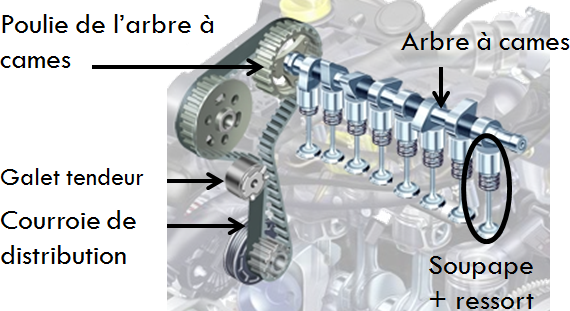
\includegraphics[height=3.5cm]{png/fig1} &
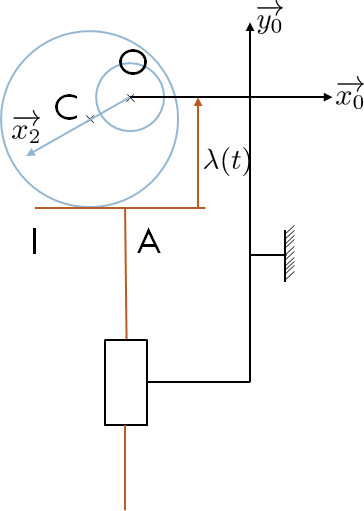
\includegraphics[height=3.5cm]{png/fig2}\\
\textit{Modèle CAO d'un} & \textit{Modélisation par}\\
 \textit{arbre à came} & \textit{schéma cinématique}\\
\end{tabular}
\end{center}


\vspace{.2cm}
Dans de nombreux mécanismes, la liaison entre deux solides est modélisée par un contact ponctuel. Cependant, l'écriture du torseur cinématique correspondant au mouvement entre les deux solides n'est pas toujours évidente. 

Intéressons nous par exemple au cas d'un système de distribution présent sur les véhicules équipés de moteurs thermiques. Ce système permet l'admission du mélange air+carburant dans la chambre de combustion et l'échappement des gaz brulés par l'intermédiaire de \textbf{soupapes}. Ces soupapes ont un mouvement de translation. L'ouverture et la fermeture des soupapes est réglée par l'intermédiaire de \textbf{cames} et d'un \textbf{arbre à cames}. La rotation de l'arbre à came est effectuée grâce à un entraînement par une courroie directement reliée au \textbf{vilebrequin} du moteur. 


\begin{prob}
\textsc{Problématique :}
\begin{itemize}
\item Comment calculer le vecteur vitesse et le vecteur instantané de rotation dans une liaison de type sphère -- plan ?
\end{itemize}
\end{prob}

%\begin{savoir}
%\textsc{Savoirs :}
%\begin{itemize}
%\item Connaître les principes de la cinématique des contacts (adhérence ou glissement, roulement et pivotement)
%\end{itemize}
%\end{savoir}

\setlength{\parskip}{0ex plus 0.2ex minus 0ex}
 \renewcommand{\contentsname}{}
 \renewcommand{\baselinestretch}{1}

\tableofcontents

 \renewcommand{\baselinestretch}{1.2}
\setlength{\parskip}{2ex plus 0.5ex minus 0.2ex}

% \vspace{1cm}
\textit{Ce document est en évolution permanente. Merci de signaler toutes
erreurs ou coquilles.}


\section{Présentation -- Système de distribution}

\begin{minipage}[c]{.65\linewidth}
Intéressons nous à la modélisation d'une soupape, notée $S_1$ en liaison glissière d'axe $(A,\vect{y_0})$ avec le moteur $S_0$. La came $S_2$ est en liaison pivot d'axe $(O,\vect{z_0})$ avec $S_0$.  $S_1$ et $S_2$ sont en liaison sphère -- plan de normale $(I,\vect{y_0})$.

L'objectif de ce cours est de calculer $\vecto{S_2}{S_1}$ et $\vect{V(I,S_2/S_1)}$.
\end{minipage}
\begin{minipage}[c]{.3\linewidth}
\begin{center}
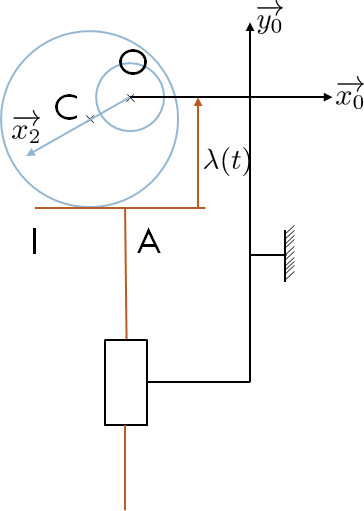
\includegraphics[width=.8\textwidth]{png/fig2} 
\end{center}
\end{minipage}
.
%\ifthenelse{\boolean{prof}}{%
%\begin{center}
%  \begin{tabular}{|>{\columncolor[gray]{.95}}p{0.6\textwidth}|}
%\hline
%$$
%\{\mathcal{V}(S_2/S_1)\}
%=\left\{
%\begin{array}{c}
%\vect{\Omega(S_2/S_1)}\\
%\vect{V(I,S_2/S_1)}
%\end{array}
%\right\}_I
%$$ \\
%\hline
%\end{tabular}
%\end{center}
%}{
%\begin{center}
%\begin{tabular}{|p{8cm}|}
%\hline
%\\
%\\
%\\
%\\
%\hline
%\end{tabular}
%\end{center}
%}


\section{Modélisation des vitesses de glissement}
\subsection{Hypothèses}
Considérons deux solides $S_1$ et $S_2$ en contact ponctuel. 

Définissons alors $I$ le point de contact entre les deux solides et $\vect{n_{12}}$ la normale de contact. On appelle $\mathcal{P}$ le plan normal à $\vect{n_{12}}$ en $I$. Il est tangent à $S_1$ et $S_2$. 

On note $\vecto{S_2}{S_1}$ le vecteur instantané de rotation entre $S_2$ et $S_1$ et $\vect{V(I,S_2/S_1)}$ le vecteur vitesse de glissement entre les deux solides.
%On note $
%\{\mathcal{V}(S_2/S_1)\}
%=\left\{
%\begin{array}{c}
%\vect{\Omega(S_2/S_1)}\\
%V(I,S_2/S_1)
%\end{array}
%\right\}_I$
%le torseur cinématique du mouvement relatif de $S_2$ par rapport à $S_1$ au point $I$.


\begin{center}
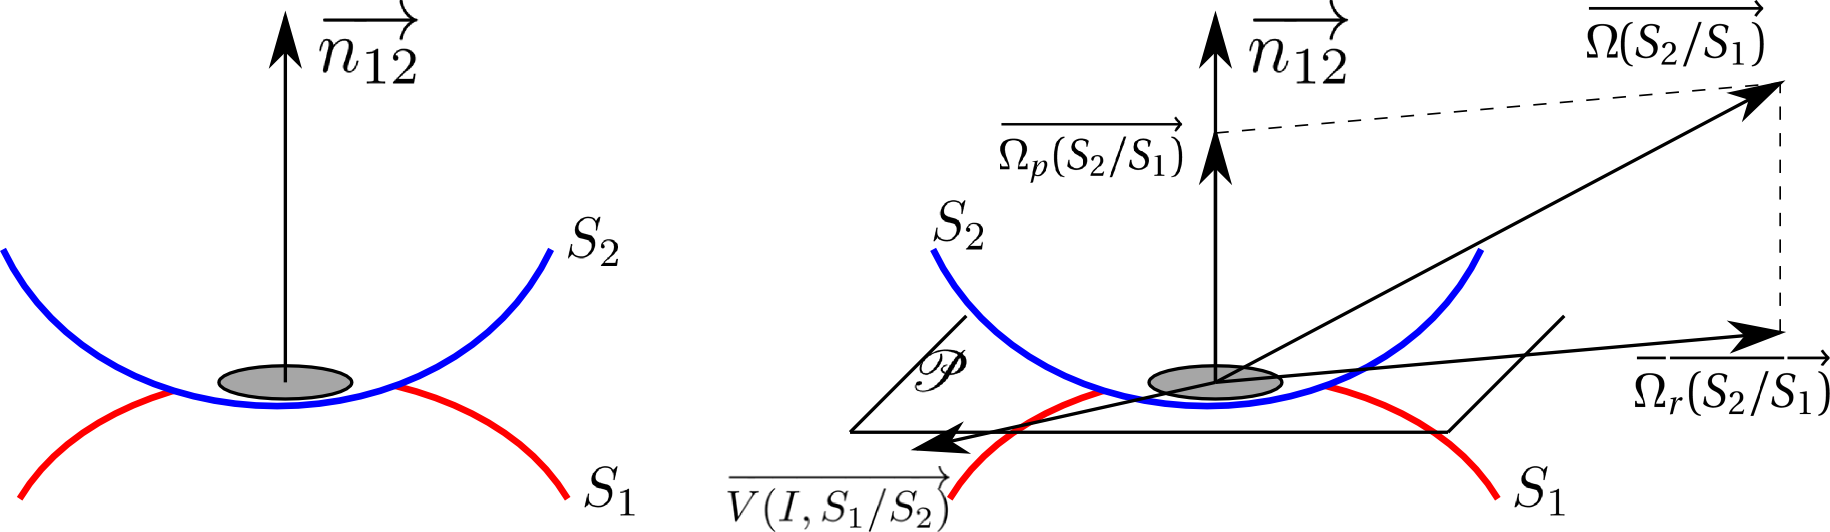
\includegraphics[width=.8\textwidth]{png/ContactReel} 
\end{center}

\subsection{Vitesses de rotation}
On a vu que dans le cas d'un contact ponctuel il existait 3 degrés de libertés de rotation paramétrables par les angles d'Euler. Nous ne cherchons pas ici à calculer directement le vecteur $\vect{\Omega(S_2/S_1)}$ en fonction de ces angles.

Cependant, ce vecteur est décomposable en une somme de deux vecteurs.
\subsubsection*{Le vecteur de pivotement}
Ce vecteur est normal au plan $\mathcal{P}$. On le note $\vect{\Omega_p(S_2/S_1)}$. On a donc :
$$
\vect{\Omega_p(S_2/S_1)} = ||\vecto{S_2}{S_1}\cdot \vect{n_{12}}||\cdot \vect{n_{12}}
$$
\subsubsection*{Le vecteur de roulement}
Ce vecteur est contenu dans le plan $\mathcal{P}$. On le note $\vect{\Omega_r(S_2/S_1)}$.


\begin{resultat}
\textbf{Vitesse de rotation}

La vitesse de rotation se compose donc ainsi :
$$\vect{\Omega(S_2/S_1)} = \vect{\Omega_p(S_2/S_1)} + \vect{\Omega_r(S_2/S_1)}$$
\end{resultat}



\subsection{Vitesse de glissement}
\subsubsection{Position du point de contact entre solides}
Cinématiquement, le point $I$ n'est pas unique. En effet, on peut distinguer l'existence de 3 points différents :
\begin{itemize}
\item le point I matériel appartenant au solide $S_1$;
\item le point I matériel appartenant au solide $S_2$;
\item le point I (non matériel) correspondant au point de contact entre les deux solides.
\end{itemize}

À l'instant $t$, ces points peuvent être confondus. À $t+dt$ ils peuvent être distincts.

En conséquence :
\begin{resultat}
$$
\vect{V(I,S_2/S_0)} \neq \vect{V(I,S_1/S_0)}
$$ 
\end{resultat}

\begin{exemple}
\begin{center}
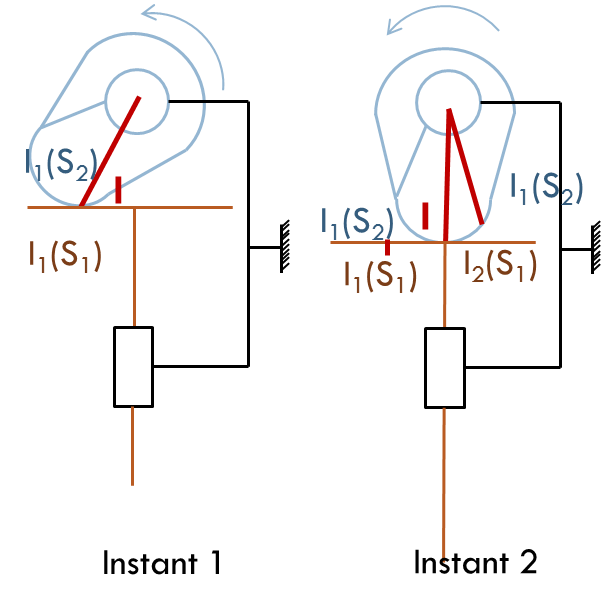
\includegraphics[width=.4\textwidth]{png/ptI}
\end{center}
\end{exemple}

\subsubsection{Définition de la vitesse de glissement}
On appelle vecteur vitesse de glissement en $I$ de $S_2/S_1$ le vecteur $\vect{V(I,S_2/S_1)}$.

\begin{rem}
On considère qu'il y a toujours contact entre $S_1$ et $S_2$ et que les solides sont indéformables. En conséquence :
$$\vect{V(I,S_2/S_1)} \in \mathcal{P}$$
\end{rem}

\subsubsection{Condition de roulement sans glissement}
\begin{defi}
\textbf{Condition de roulement sans glissement}

Dans de très nombreux mécanismes (dans les engrenages, lors du contact entre la roue et le sol \textit{etc}) on peut faire l'hypothèse que le glissement est nul. On a alors : 

$$
\vect{V(I,S_2/S_1)} = \vect{0}
$$
\end{defi}


Il est alors possible d'identifier des lois de comportement.
\subsection{Méthode de calcul de la vitesse de glissement}
Le calcul de la vitesse de glissement peut se calculer à l'aide de la procédure suivante.

\begin{methode}
\begin{enumerate}
\item Paramétrer le système
\item Décomposer le mouvement : $\vect{V(I,S_1/S_2)}=\vect{V(I,S_1/S_0)}+\vect{V(I,S_0/S_2)}$
\item Calculer $\torseurcin{V}{S_1}{S_0}$ au point $I$
\item Calculer $\torseurcin{V}{S_2}{S_0}$ au point $I$
\item Calculer  $\vect{V(I,S_1/S_2)}$
\end{enumerate}
\end{methode}

\begin{warn}
\textbf{$I$ n'est pas un point matériel. Il n'appartient ni à $S_1$ ni à $S_2$. On ne peut donc pas calculer $\left[\dfrac{\vect{OI}}{dt}\right]_{\mathcal{R}_0}$}.
\end{warn}

%\newpage

\section{Application -- Calcul de la vitesse de glissement entre la came et la soupape}
Pour le système de distribution composé d'une came, d'une soupape et du moteur, on se propose de calculer la vitesse de glissement entre la soupape et la came.
\subsection*{Paramétrage}
\begin{center}
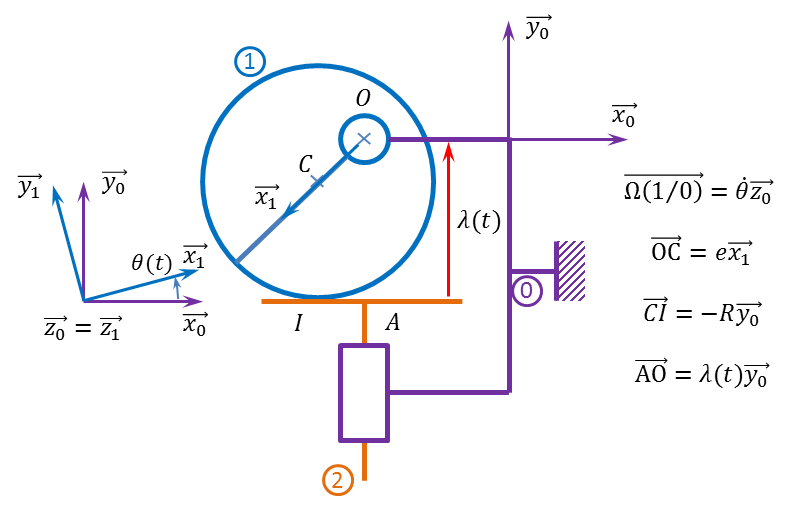
\includegraphics[width=.7\textwidth]{png/parametrage} 
\end{center}

\subsection*{Détermination de la loi Entrée -- Sortie}
La fermeture géométrique de la chaîne est : 
$$
\vect{OC}+\vect{CI}+\vect{IA}+\vect{AO} = \vect{0} \Longleftrightarrow e\vect{x_1} -R\vect{y_0} + \mu(t)\vect{x_0}+\lambda(t) \vect{y_0} = \vect{0}
$$

L'équation en projection sur $\vect{y_0}$ est la suivante : 
$$
e\vect{x_1}\cdot \vect{y_0} -R +\lambda(t)  = 0 
\Longleftrightarrow e\cos\left(\dfrac{\pi}{2}-\theta \right) -R +\lambda(t)  = 0
\Longleftrightarrow e\sin \theta -R +\lambda(t)  = 0
$$

La loi en vitesse est donc donnée par :
$$
e\dot{\theta}\cos \theta +\dot{\lambda}(t)  = 0
$$

\subsection*{Décomposition en mouvements simples}
D'après la composition des mouvements, on a : 
$$
\vect{V(I,S_1/S_2)} = \vect{V(I,S_1/S_0)} + \vect{V(I,S_0/S_2)}
= \vect{V(I,S_1/S_0)} - \vect{V(I,S_2/S_0)}
$$

%\begin{center}
%\begin{tabular}{|p{8cm}|}
%\hline
%$$
%\vect{V(I,S_2/S_1)} = \vect{V(I,S_1/S_0)} + \vect{V(I,S_0/S_2)}
%$$
%\\
%\hline
%\end{tabular}
%\end{center}

%\subsection*{Calcul de $\{\mathcal{V}(S_1/S_0)\}$}
\subsection*{Calcul de $\vect{V(I,S_2/S_0)}$}
Nature du mouvement entre $S_2$ et $S_0$ : liaison glissière d'axe $(A,\vect{y_0})$.
On a donc :

$$
\begin{array}{l}
\vect{\Omega(S_2/S_0)} = \vect{0} \\
\vect{V(A,S_2/S_0)} = \left[\dfrac{d\vect{OA}}{dt}\right]_{\mathcal{R}_0}  = -\dot{\lambda}(t) \vect{y_0}\\
\end{array}
$$

%$$
%\{\mathcal{V}(S_1/S_0)\} =
%\left\{
%\begin{array}{c}
%\vect{\Omega(S_1/S_0)} = \vect{0} \\
%\vect{V(A,S_1/S_0)} = \dfrac{d\vect{OA}}{dt} \\
%\end{array}
%\right\}_A
%$$

%Calculons $\vect{V(A,S_1/S_0)}$ :
%$$
%\vect{V(A,S_1/S_0)} = \dfrac{d\vect{OA}}{dt} = \dfrac{d\lambda(t)\vect{y_0}}{dt} =  e \dot{\theta}(t) \cos \theta(t) \vect{y_0}
%$$

Calculons alors $\vect{V(I,S_2/S_0)}$ :
$$ \vect{V(I,S_2/S_0)} = \vect{V(A,S_2/S_0)} + \underbrace{\vect{IA} \wedge \vect{\Omega(S_2/S_0)}}_{\vect{0}} $$
%
%D'où :
%\begin{center}
%\begin{tabular}{|p{8cm}|}
%\hline
%$$
%\{\mathcal{V}(S_1/S_0)\} =
%\left\{
%\begin{array}{c}
%\vect{\Omega(S_1/S_0)} = \vect{0} \\
%\vect{V(I,S_1/S_0)} = e \dot{\theta}(t) \cos \theta(t) \vect{y_0}  \\
%\end{array}
%\right\}_I
%$$
%\\
%\hline
%\end{tabular}
%\end{center}

%\subsection*{Calcul de $\{\mathcal{V}(S_2/S_0)\}$}
\subsection*{Calcul de $\vect{V(I,S_1/S_0)}$}
Nature du mouvement entre $S_1$ et $S_0$ : liaison pivot d'axe $(O,\vect{z_0})$.
On a donc : 

$$
%\{\mathcal{V}(S_2/S_0)\} =
%\left\{
\begin{array}{l}
\vect{\Omega(S_1/S_0)} = \dot{\theta}\vect{z_0} \\
\vect{V(A,S_1/S_0)} = \vect{0} \\
\end{array}
%\right\}_O
$$

Calculons alors $\vect{V(I,S_1/S_0)}$ :
$$
\vect{V(I,S_1/S_0)} 
= \underbrace{\vect{V(O,S_1/S_0)}}_{\vect{0} }
+ \vect{IO} \wedge \vect{\Omega(S_1/S_0)} = \left(R\vect{y_0}-e\vect{x_1}\right) \wedge \dot{\theta}\vect{z_0}
= R\dot{\theta}\vect{x_0} + e\dot{\theta}\vect{y_1}
$$

%$$
%\vect{V(I,S_2/S_0)} = R\dot{\theta}\vect{x_0} + e\dot{\theta}\vect{y_2}
%$$
%
%D'où :
%\begin{center}
%\begin{tabular}{|p{8cm}|}
%\hline
%$$
%\{\mathcal{V}(S_2/S_0)\} =
%\left\{
%\begin{array}{c}
%\vect{\Omega(S_2/S_0)} = \dot{\theta}\vect{z_0} \\
%\vect{V(I,S_2/S_0)} = R\dot{\theta}\vect{x_0} + e\dot{\theta}\vect{y_2}  \\
%\end{array}
%\right\}_I
%$$ \\
%\hline
%\end{tabular}
%\end{center}

\subsection*{Calcul de $\vect{V(I,S_1/S_2)}$}

Au final, on a :
$$
\vect{V(I,S_1/S_2)} = \vect{V(I,S_1/S_0)} - \vect{V(I,S_2/S_0)}
= R\dot{\theta}\vect{x_0} + e\dot{\theta}\vect{y_1} +\dot{\lambda}(t) \vect{y_0}
$$

En projetant $\vect{y_1}$ dans $\mathcal{R}_0$ : 
$$
\vect{V(I,S_1/S_2)} 
= R\dot{\theta}\vect{x_0} + e\dot{\theta}\left( \cos\theta \vect{y_0} - \sin\theta \vect{x_0} \right)+\dot{\lambda}(t) \vect{y_0} 
= \left(R\dot{\theta} - e\dot{\theta}\sin\theta \right) \vect{x_0} + \left(e\dot{\theta} \cos\theta +\dot{\lambda}(t) \right) \vect{y_0}
$$

Or, d'après la loi entrée-sortie, $e\dot{\theta}\cos \theta +\dot{\lambda}(t)  = 0$. (On pourrait aussi remarquer que la vitesse de glissement est contenue dans le plan tangent au contact).

On a donc :
$$
\vect{V(I,S_1/S_2)} 
= \dot{\theta}\left(R - e\sin\theta \right) \vect{x_0} 
$$

%
%$$
%\vect{V(I,S_2/S_1)} = \vect{V(I,S_1/S_0)} + \vect{V(I,S_0/S_2)}
%$$
%
%$$
%\Longleftrightarrow \vect{V(I,S_2/S_1)} = \vect{V(I,S_1/S_0)} - \vect{V(I,S_2/S_0)}
%$$
%
%$$
%\Longleftrightarrow \vect{V(I,S_2/S_1)} =  e \dot{\theta}(t) \cos \theta(t) \vect{y_0} - \left( R\dot{\theta}\vect{x_0} + e\dot{\theta}\vect{y_2} \right)
%$$
%
%$$
%\Longleftrightarrow \vect{V(I,S_2/S_1)} = 
% e \dot{\theta}(t) \cos \theta(t) \vect{y_0} 
%- R\dot{\theta}\vect{x_0} 
%- e\dot{\theta}\left( \cos \theta(t) \vect{y_0}- \sin \theta(t) \vect{x_0} \right)
%$$
%
%Au final :
%\begin{center}
%\begin{tabular}{|p{8cm}|}
%\hline
%$$
%\vect{V(I,S_2/S_1)} =  \dot{\theta}\left(e\sin \theta(t) - R\right)\vect{x_0} 
%$$\\
%\hline
%\end{tabular}
%\end{center}


\section{Calcul du rapport de transmission d'un engrenage}
\subsection{Étude d'un convoyeur à bande}
\begin{exemple}
\begin{minipage}[c]{.55\linewidth}
Un convoyeur à bande est un dispositif de transport de manutention permettant le déplacement continue de marchandises en vrac ou de charges isolées. Il est constitué essentiellement d'une bande sans fin (ou courroie) en matériau souple entraînée par un tambour moteur. La bande, plus ou moins large, comporte un brin inférieur et un brin supérieur, lequel supporte et entraîne les marchandises posées dessus.
\end{minipage}\hfill
\begin{minipage}[c]{.4\linewidth}
\begin{center}
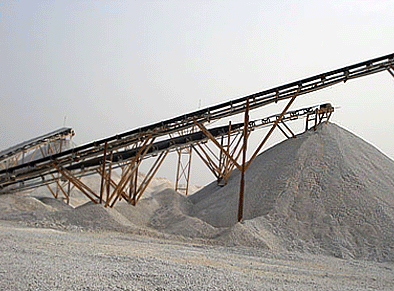
\includegraphics[width=.9\textwidth]{png/fig02}
\end{center}
\end{minipage}
\end{exemple}

L'objectif est de calculer le rapport de réduction du tambour moteur. 


Les engrenages sont représentables ainsi :
\begin{center}
\begin{minipage}[c]{.2\linewidth}
\begin{center}
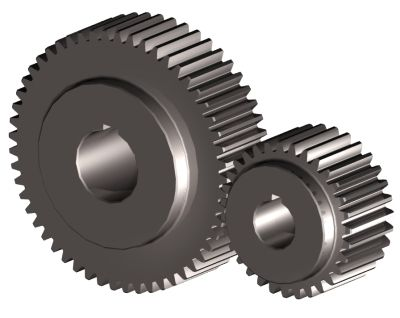
\includegraphics[height=3cm]{png/fig3}
\textit{Engrenage}
\end{center}
\end{minipage} \hfill
\begin{minipage}[c]{.3\linewidth}
\begin{center}
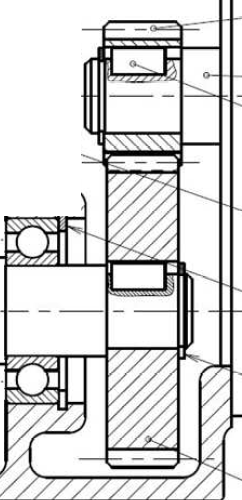
\includegraphics[height=5cm]{png/fig4}

\textit{Représentation 2D}
\end{center}
\end{minipage} \hfill
\begin{minipage}[c]{.3\linewidth}
\begin{center}
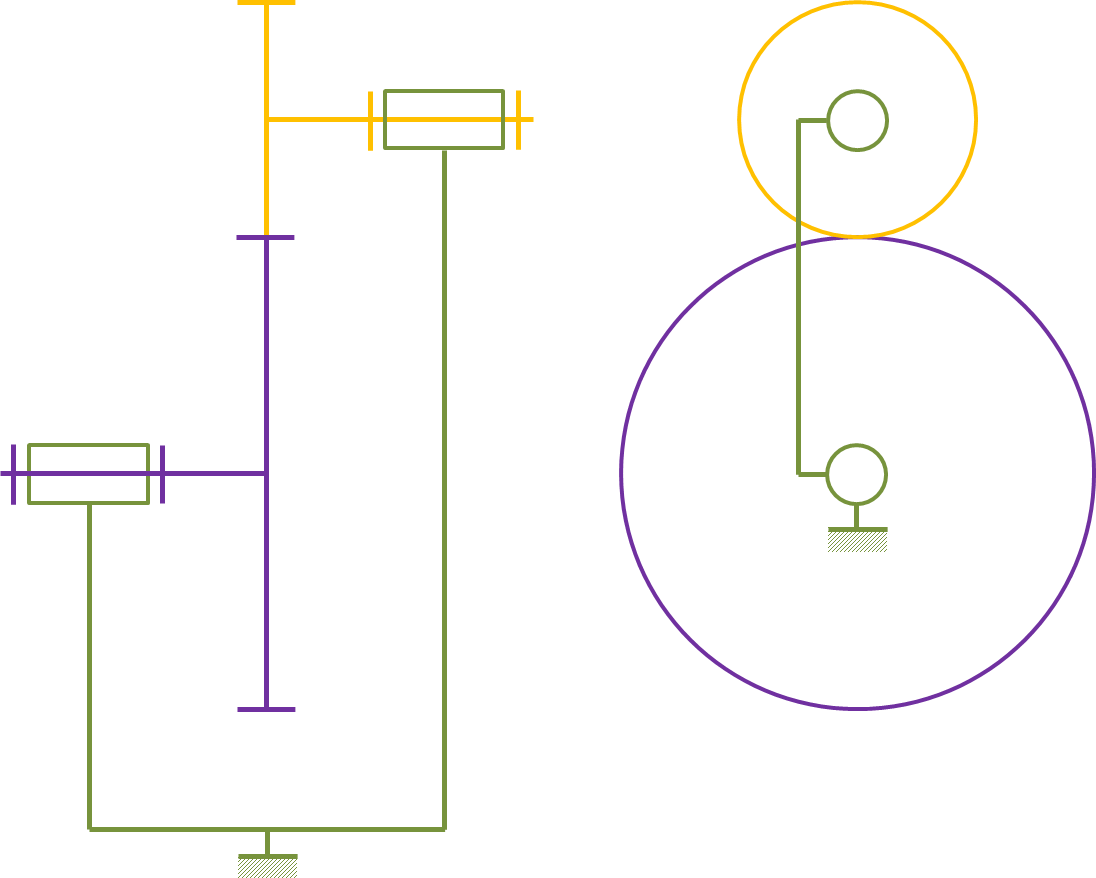
\includegraphics[height=5cm]{png/fig5}

\textit{Schéma cinématique}
\end{center}
\end{minipage} \hfill
\end{center}

\begin{center}
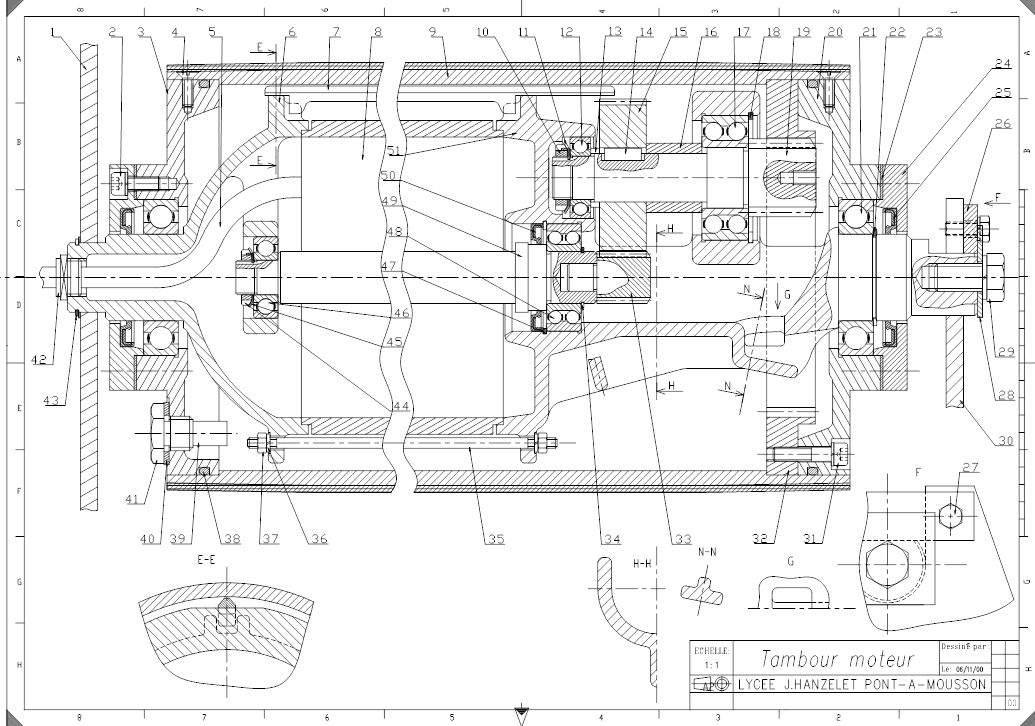
\includegraphics[width=.95\textwidth]{png/fig01}
\end{center}

On donne :
\begin{itemize}
\item $Z_{33}=16$ et $m=1,5$;
\item $Z_{15}=59$ et $m=1,5$;
\item $Z_{19}=17$ et $m=2,5$;
\item $Z_{32}=62$ et $m=2,5$.
\end{itemize}

\begin{enumerate}
\item Réaliser le schéma cinématique minimal du moteur tambour.
\item Réaliser le paramétrage du système.
%\item A l'aide de votre GDI, déterminer ce qu'est le module d'un engrenage ainsi que le diamètre primitif. Donner alors la relation existant entre le module, le diamètre primitif et le nombre de dents.
\item En utilisant l'hypothèse de roulement sans glissement entre les pièces 33 et 15, déterminer le rapport de réduction $r_1=\dfrac{\omega(19/1)}{\omega(33/1)}$.
\item En utilisant l'hypothèse de roulement sans glissement entre les pièces 33 et 15, déterminer le rapport de réduction $r_2=\dfrac{\omega(9/1)}{\omega(19/1)}$.
\item En déduire alors le rapport de réduction du réducteur : $r=\dfrac{\omega(9/1)}{\omega(33/1)}$.
\end{enumerate}

\subsection{Rapport de transmission dans un train d'engrenages}
\begin{defi}
\begin{minipage}[c]{.55\linewidth}
Un engrenage est réalisé par la mise en contact de deux roues dentées. Parmi l'ensemble des paramètres existants, on retiendra l'existence d'un diamètre primitif, et l'existence d'un module.

Dans le fonctionnement d'un engrenage, les deux roues dentées roulent sans glisser l'une par rapport à l'autre selon leur cylindre primitif. 

Pour engrener, les roues dentées doivent avoir le même module.

En notant $m$ le module, $Z$ le nombre de dents et $d_p$ le diamètre primitif d'une roue dentée, on a :
$$
d_p = mZ
$$
\end{minipage} \hfill
\begin{minipage}[c]{.4\linewidth}
\begin{center}
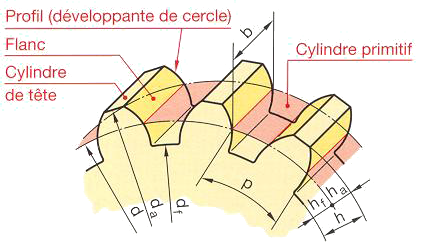
\includegraphics[width=.95\textwidth]{png/gdi}

\textit{D'après GDI -- Engrenages \cite{gdi}}
\end{center}
\end{minipage}
\end{defi}

\begin{resultat}
Dans un train d'engrenage, en utilisant le formalisme des fonctions de transfert, le rapport de réduction peut être défini ainsi : 
$$
r = \dfrac{\omega_{\text{sortie/bâti}}}{\omega_{\text{entrée/bâti}}} =  \left(-1\right)^n\dfrac{\prod Z_{\text{menantes}}}{\prod Z_{\text{menées}}}
$$
\end{resultat}

%\begin{rem}
%Il existe aussi la notion de rapport de transmission. Dans la norme la valeur absolue de ce rapport 
%\end{rem}

\section{Calcul du rapport de transmission dans un train épicycloïdal}
\subsection{Étude d'un compensateur de bulldozer}
\begin{exemple}
\begin{minipage}[c]{.55\linewidth}

Un train compensateur est un élément de transmission de puissance que l'on retrouve sur les bulldozer. Il permet notamment d'adapter la vitesse de rotation délivrée par le moteur pour les roues motrices des chenilles droites et gauches.

L'objectif de cette étude est de vérifier une performance du réducteur et du train compensateur dont on donne un extrait du cahier des charges fonctionnel ainsi que le dessin d'ensemble. 

On donne $Z_{25}=32$, $Z_{23}=23$, $Z_{17}=78$.
\end{minipage}\hfill
\begin{minipage}[c]{.4\linewidth}
\begin{center}
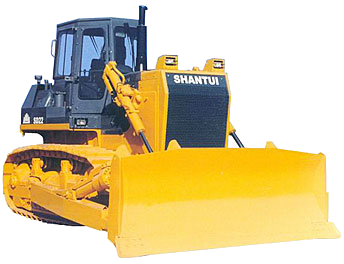
\includegraphics[width=.9\textwidth]{png/fig7}
\end{center}
\end{minipage}
\end{exemple}

\begin{minipage}[c]{.4\linewidth}

\begin{enumerate}
\item Identifier les classes d'équivalence cinématique sur le dessin d'ensemble puis réaliser le schéma cinématique et le paramétrage du système.
\item Après avoir écrit la relation de roulement sans glissement entre les roues 23 et 24 donner une relation entre $\omega_{23/28}$, $\omega_{25/17}$, $\omega_{28/17}$ et les paramètres géométriques des engrenages.
\item Après avoir écrit la relation de roulement sans glissement entre les roues 23 et 17 donner une relation entre $\omega_{23/28}$, $\omega_{28/17}$ et les paramètres géométriques des engrenages.
\item En déduire le rapport de réduction du train épicycloïdal : $\dfrac{\omega_{28/17}}{\omega_{25/17}}$.
\item Donner une relation géométrique de fonctionnement entre les différents paramètres géométriques des engrenages.
\end{enumerate}
\end{minipage}\hfill
\begin{minipage}[c]{.55\linewidth}
\begin{center}
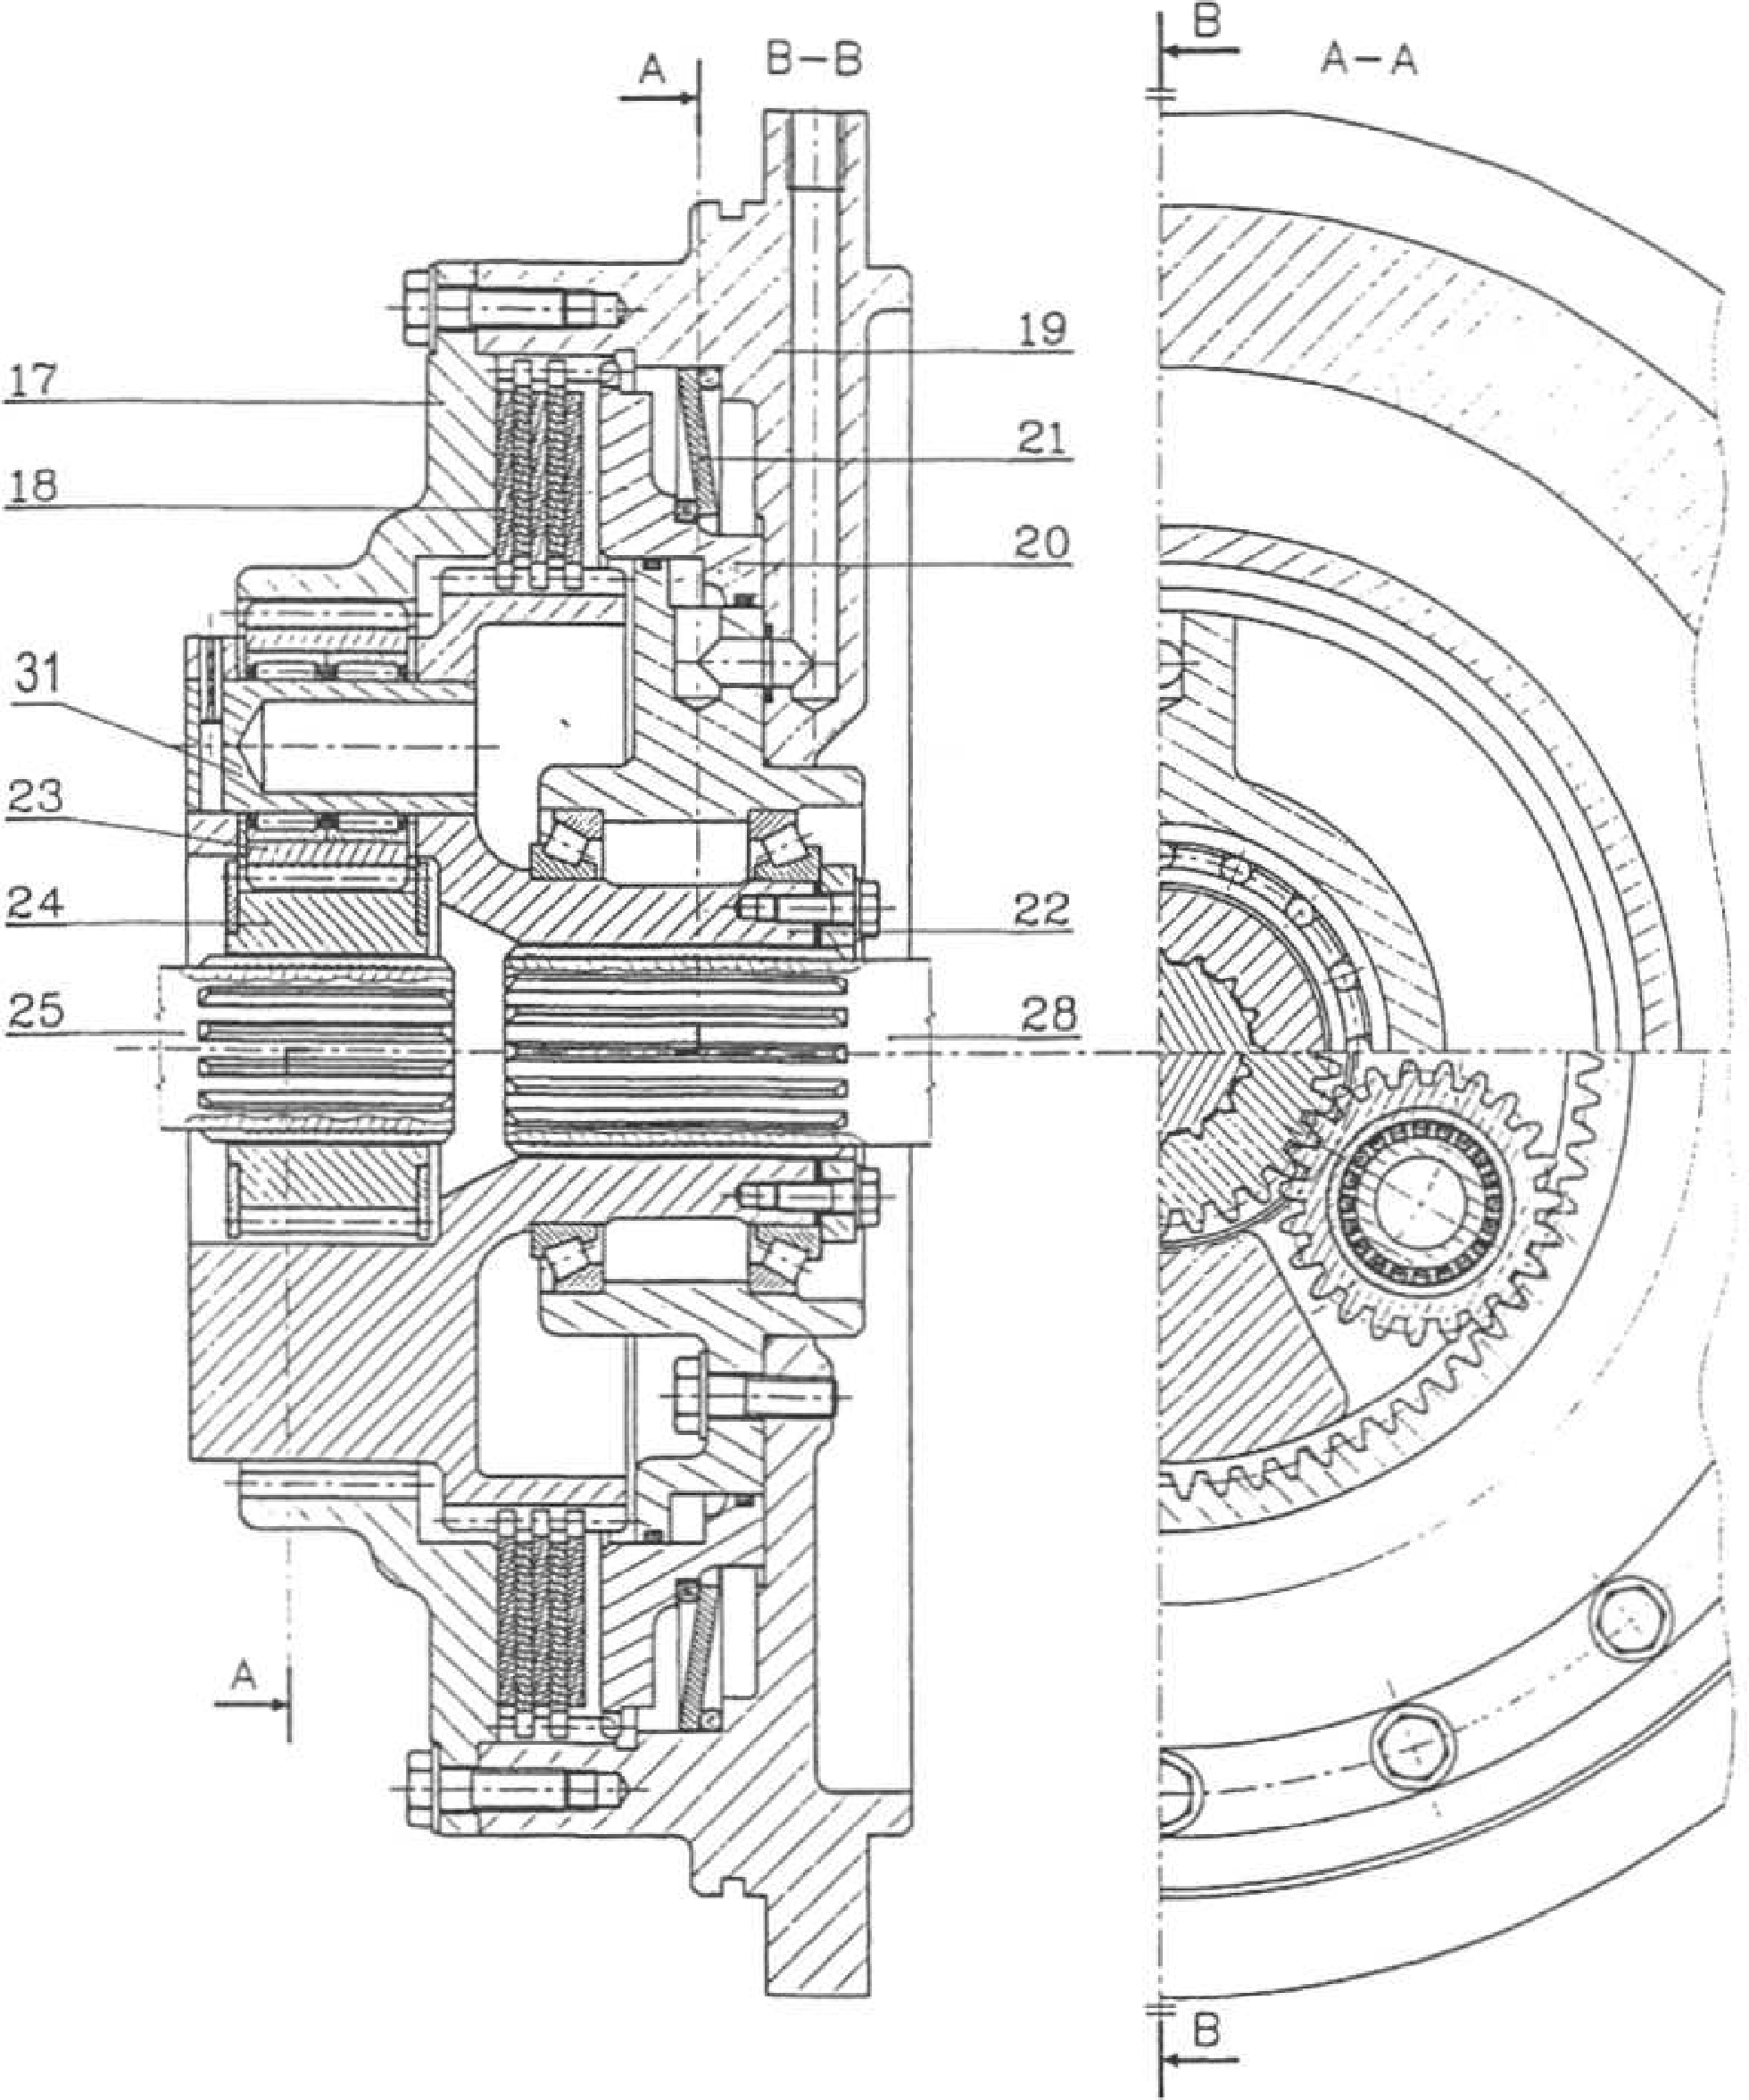
\includegraphics[width=.95\textwidth]{png/fig9}
\end{center}
\end{minipage}

\subsection{Méthode générale de calcul de rapport du rapport de transmission dans un train épicycloïdal}

\begin{methode}
\begin{enumerate}
\item On trace le graphe de structure.
\item On écrit la condition de roulement sans glissement au point $I$. 
\item On établit une première relation entre les taux de rotation en utilisant le décomposition du vecteur vitesse.
\item On écrit la condition de roulement sans glissement au point $J$.
\item On établit une seconde relation  entre les taux de rotation en utilisant le décomposition du vecteur vitesse.
\item On combine les deux relations obtenues pour avoir une relation entre les taux de rotation.
\item Si nécessaire, on utilise la décomposition du taux de rotation pour avoir le rapport de réduction final.
\end{enumerate}
\end{methode}


\begin{thebibliography}{2}
\bibitem[1]{gdi} André Chevalier, Guide du dessinateur Industriel, Éditions Hachette Technique.
\end{thebibliography}
\end{document}


\end{document}


